\documentclass[11pt]{article}
\usepackage[a4paper,total={170mm,257mm},left=10mm,right=10mm,top=20mm,bottom=10mm]{geometry}
\usepackage[T1]{fontenc}
\usepackage[utf8]{inputenc}
\usepackage{geometry}
\usepackage{fancyhdr}
\usepackage{enumitem}
\usepackage{titlesec}
\usepackage{multicol}
\usepackage{graphicx}
\usepackage{hyperref}

\hypersetup{
    colorlinks=false,
    linkcolor=red,
    filecolor=magenta,      
    urlcolor=white,
    pdfpagemode=FullScreen,
}

\renewcommand{\headrulewidth}{.4mm} % header line width

\titleformat*{\section}{\Huge\bfseries}
\titleformat*{\subsection}{\normalsize\bfseries}
\titleformat*{\subsubsection}{\normalsize\bfseries}
\titleformat*{\paragraph}{\normalsize\bfseries}
\titleformat*{\subparagraph}{\normalsize\bfseries}

\titlespacing\section{0pt}{0pt}{-5pt}
\titlespacing\subsection{0pt}{0pt}{0pt}

\setlength{\tabcolsep}{0pt} % Remove horizontal space between columns
\renewcommand{\arraystretch}{0} % Remove vertical space between rows

\setlist{nolistsep}

\pagestyle{fancy}
\fancyhf{}
\fancyhfoffset[L]{0cm} % left extra length
\fancyhfoffset[R]{0cm} % right extra length
\rhead{+(1) 780-206-8004 \\ jcbrown1@ualberta.ca}
\lhead{\bfseries Joshua Brown, BSc. Mechanical Engineering \\ \today}
\rfoot{}

\begin{document}
\section*{Vision Based Pose Estimation \small (In Progress)}
\subsection*{What}
This last summer I worked in the mechatronic system lab at the University of Alberta. While working there I noticed that three of the graduate students working there were interested in using a vision based 6D pose detection algorithm, and they were using an old students semi-working code. I noticed that the pose detection system as I found it was not able to be extended easily to new objects, didn't work when the target objects at most orientations, and required manually labelling images to train a machine learning model. I decided to use this as an opportunity to improve a fundamental system used in the lab. 
\subsection*{How}
I used a Vicon motion capture system to locate a camera and target drone in 3D space. I then calibrated the intrinsic and extrinsic parameters of the camera so I could accurately project 3D points in the world to 2D points in an image. I used this functionality to project 8 points relative to the target drone into the image, and saved this data. A pretrained keypoint RCNN model was fine tuned on my generated data, so that I would be able to use PyTorch to estimate target drone image points on new images. The perspective-n-point algorithm implemented in OpenCV was used to convert the image points into an estimated position and orientation of a target drone
% \subsection*{Key Contributions/Responsibilities}
\subsection*{Key Technologies}
\begin{itemize}
    \item \textbf{ROS2} was used for easily making all of the different processes work together as a single system
    \item \textbf{PyTorch} was used for training and using a fine-tuned keypoint RCNN model
    \item \textbf{OpenCV} was used for calibrating the intrinsic and extrinsic matrices of the camera, projecting 3D points from the motion capture system to the image for training data, and for converting estimated image points to an estimated pose
\end{itemize}
\subsection*{Results}
This system is implemented on a cheap drone with a camera. It has been tested and used in the mechatronic system lab at the University of Alberta, and it is intended to be used by graduate students to build their own projects. The system is overall easy to use, and is not camera or target drone specific. A full 6D pose detection model can be trained in a sigle day to extend the types of drones that are to be detected. This work is currently being turned into a research paper, and will be finished by the end of the year. The code for this project is intened to be improved for use as an open source package, but is not fully ready for public use yet.

\vspace{-6mm}
\begin{center}
    \begin{tabular}{cc}
        \multicolumn{2}{c}{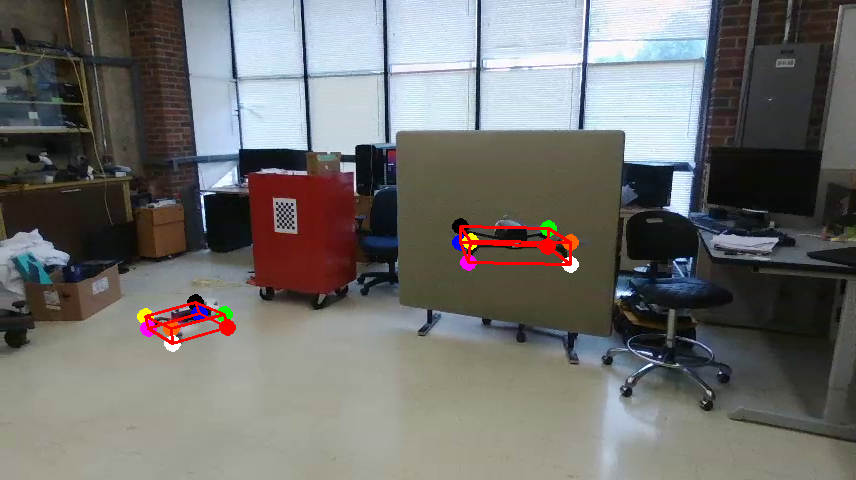
\includegraphics[width=\textwidth, trim={0mm, 35mm, 0mm, 60mm}, clip]{images/pose_detection_picture.png}}\\
        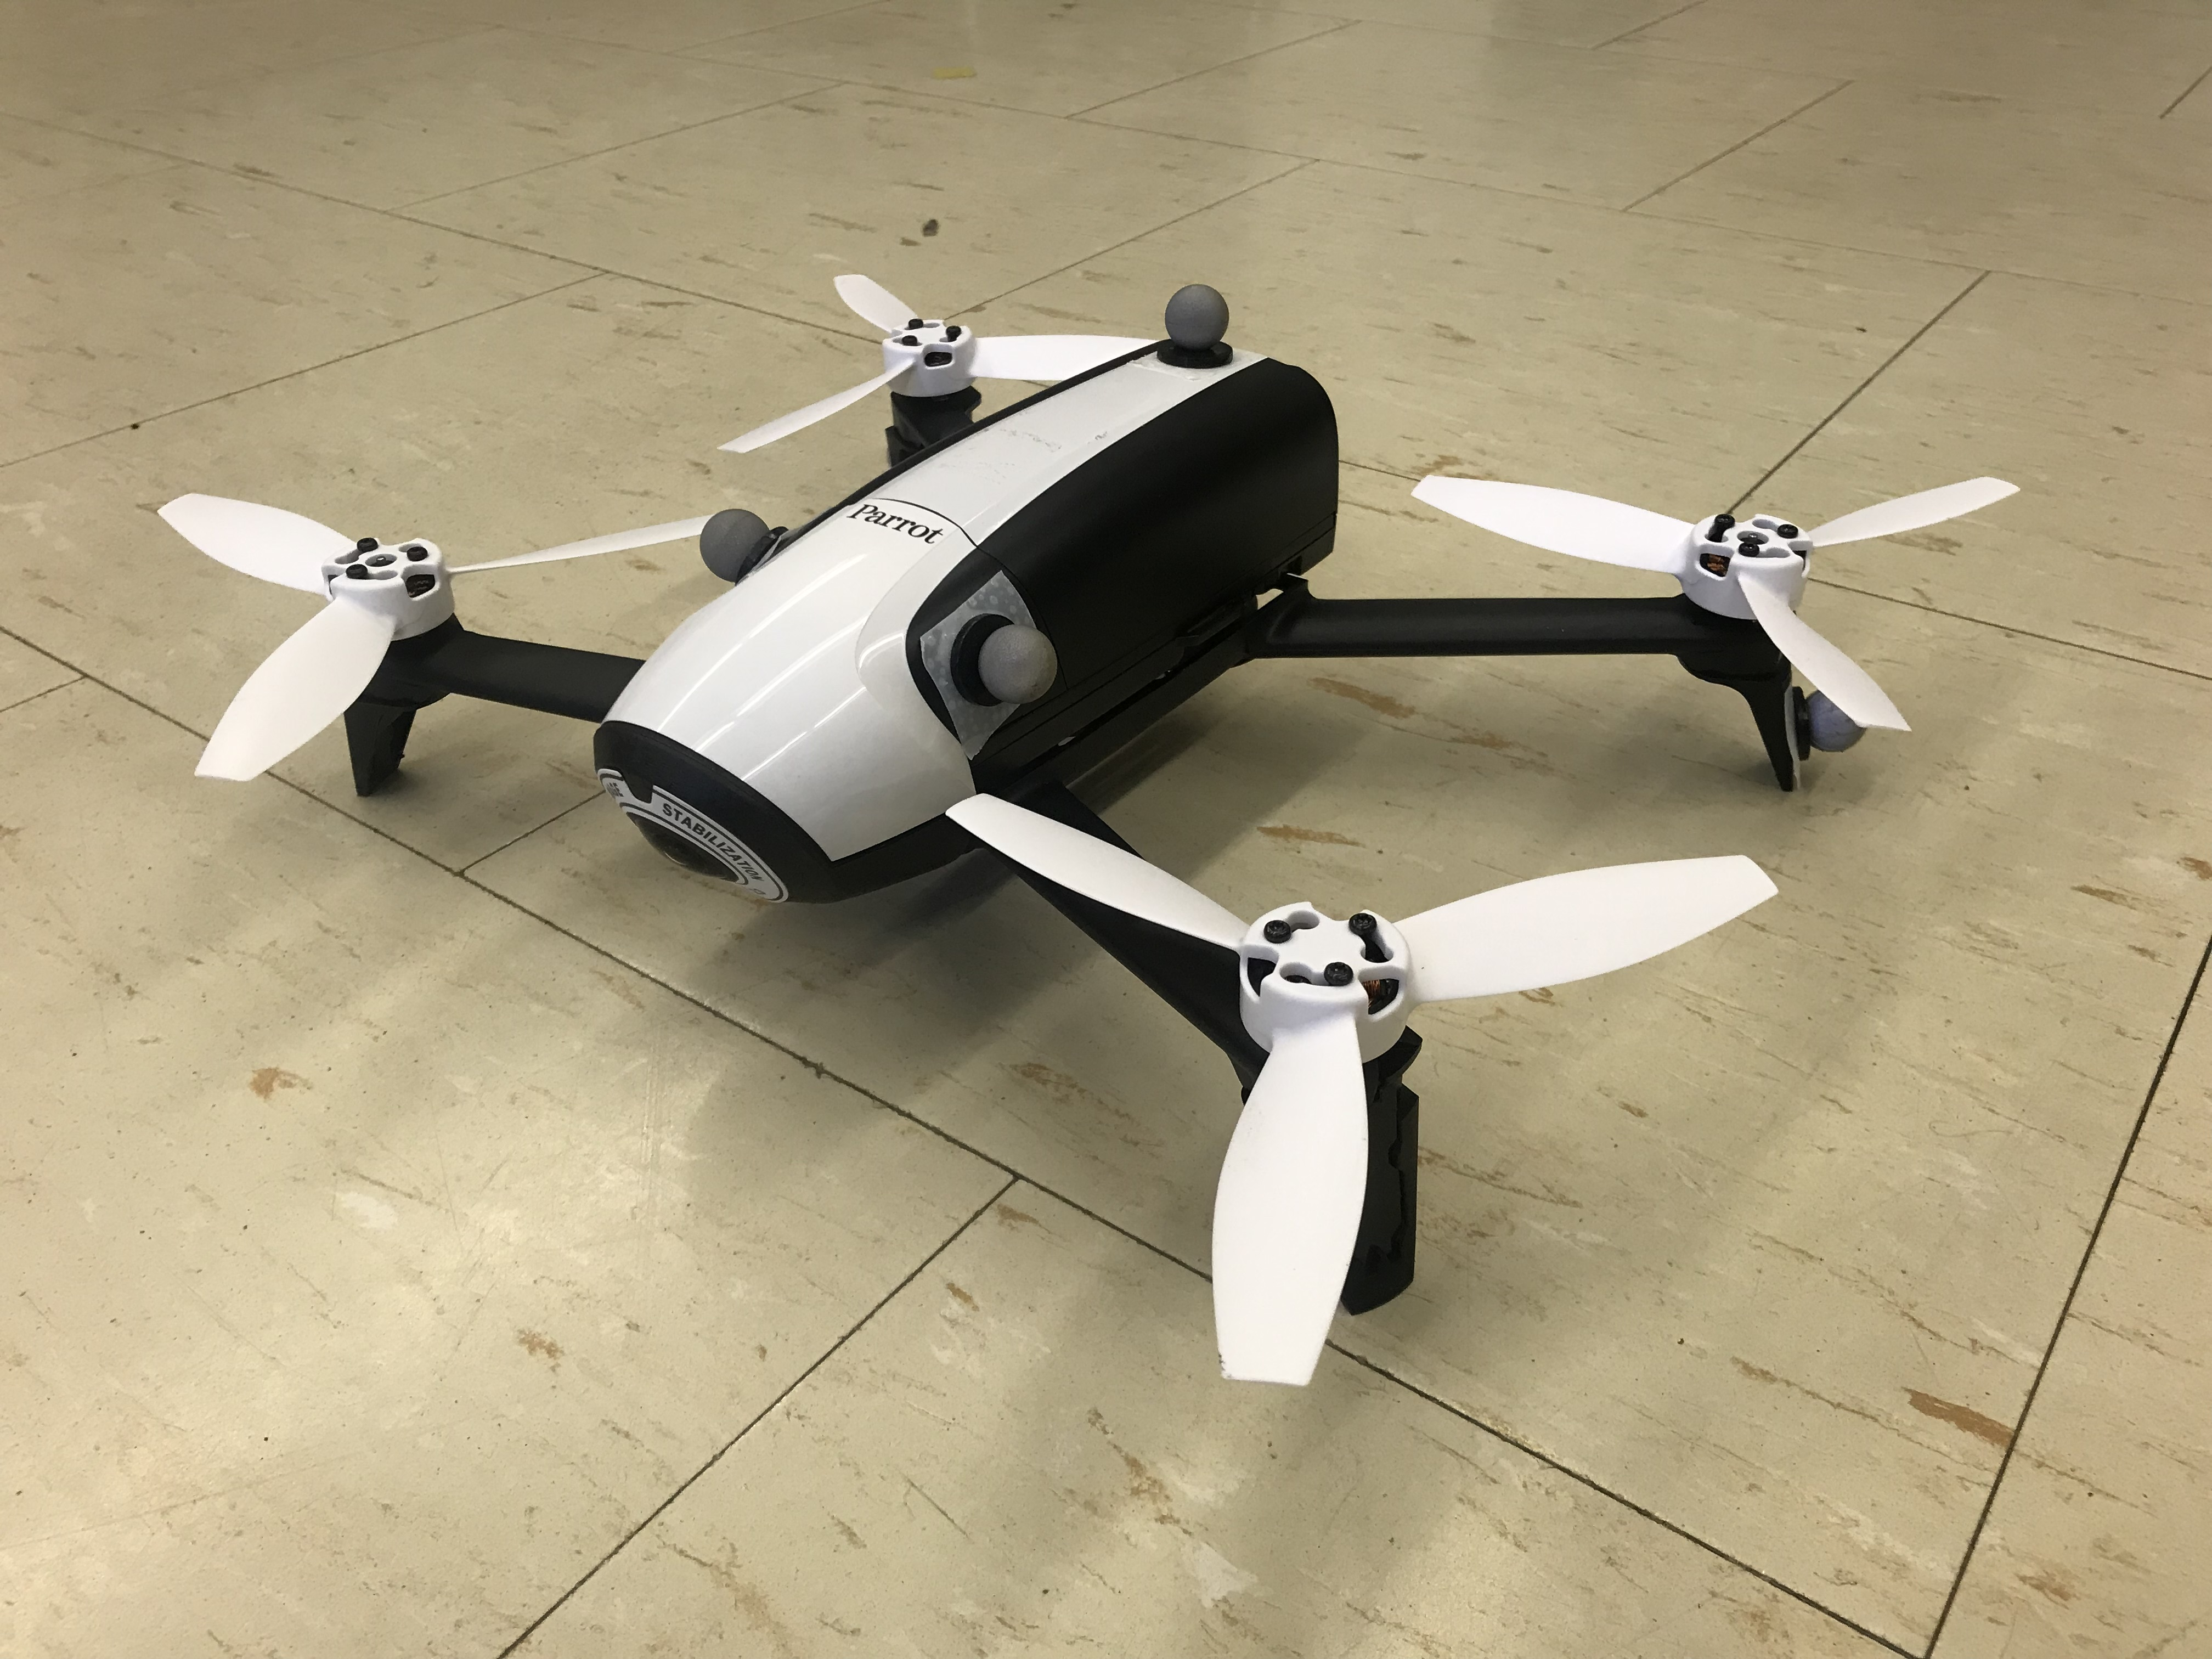
\includegraphics[width=0.54\textwidth, trim={50mm, 100mm, 100mm, 100mm}, clip]{images/bebop2_with_motion_balls.jpg} & 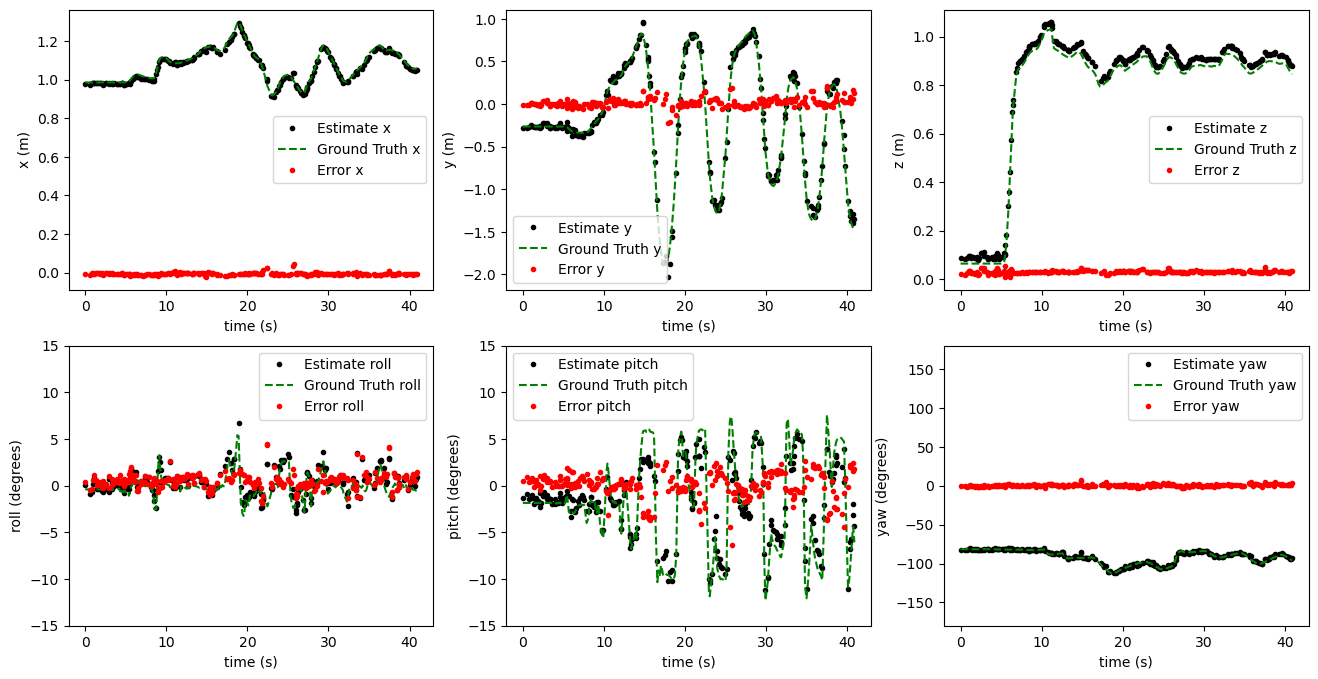
\includegraphics[width=0.46\textwidth, trim={111mm, 86mm, 113mm, 0 mm}, clip]{images/pose_detection_front_back_movement_plot.png} \\
    \end{tabular}
\end{center}
\newpage

\section*{Autonomous Robotic Vehicle Project (ARVP)}
\subsection*{What}
ARVP is an engineering club at the University of Alberta run by undergraduate students. The purpose of the club is to learn about autonomous vehicles through making a custom robot. In recent history, ARVP has been foucussed specifically on underwater robotics and competes yearly at robosub. The robot is expected to operate at $\sim 5$m of depth. It is powered by Li-ion batteries, uses $8$ thrusters for motion, has custom toy torpedo, dropper, and claw systems, and utilized a doppler velocity log (DVL) and inertial measurement unit (IMU). The team has weekly work sessions every week and operates all year, while also fitting in outreach opportunities with the community and nearby high schools. 
\subsection*{How}
Most of my time in ARVP was in the position of one of two software team leads. I worked on planning the software team's yearly goals, I worked with team members to solve technical problems that came up with their tasks, and I onboarded new members to join our team. I also lead some projects directly. While my main focus was working with the software team, I would also work with the mechanical and electrical teams. I spent time debugging and testing networking issues and CAN bus with the electrical team, and would sometimes assist and contribute to solving issues like misfiring torpedo systems.    
\subsection*{Key Responsibilities}
\begin{itemize}
    \item Lead and managed a software team's projects, onboarding, and codebase with another person
    \item Implemented a Kalman filter to estimate an AUV's state by combining DVL (velocity) and IMU sensor data 
    \item Troubleshooted network, CAN, and ROS communications live while leading full system tests
    \item Collaborated with members on technical approaches to problems, and implementation problems
\end{itemize}
\subsection*{Results}
\begin{itemize}
    \item Using the current robot Arctos, we were the top placing team in North America out of 40+
    teams at RoboSub 2023
    \item Programmed a robot to estimate its full position and orientation from sensors
    \item Lead a software team to create a robot capable of navigating and controlling itself underwater
\end{itemize}

I am the person using the computer in the top image. The team's website is here: \url{http://arvp.org}

\vspace{-6mm}
\begin{center}
    \begin{tabular}{cc}
        \multicolumn{2}{c}{\includegraphics[width=\textwidth, trim={0mm, 55mm, 0mm, 200mm}, clip]{images/arvp.png}}\\
        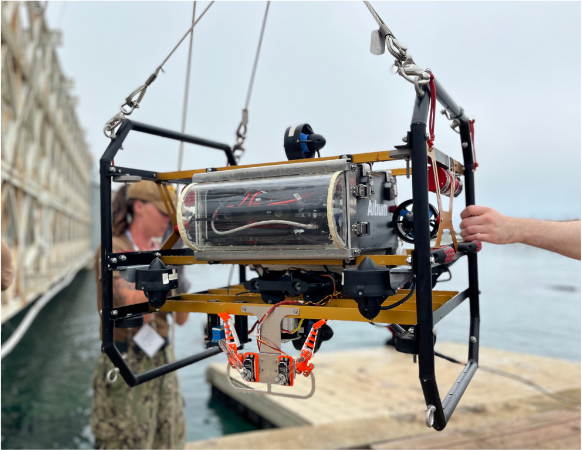
\includegraphics[width=0.5\textwidth, trim={0mm, 0mm, 0mm, 0mm}, clip]{images/arctos.png} & \includegraphics[width=0.5\textwidth, trim={30mm, 0mm, 5mm, 0mm}, clip]{images/octagon.jpg} \\
    \end{tabular}
\end{center}
\newpage

\section*{Custom Wheeled Mobile Robot}
\subsection*{What}
Through my experience as a mechanical engineering student I had an understanding of mechanical design, and as a leader in ARVP I had an understanding of software for robotics. However, I did not have any experience designing and making a full system from scratch. To solve this, I decided to make a cleaning robot. The robot uses a differential drive to drive and turn. It is entirely controlled by an arduino and, and uses an ultrasonic sensor to measure how far away the nearest wall is from it. I attached a wet wipe to the back of the robot to drag along the floor. The robot is able to detect walls and avoid them while travelling in a room. 
\subsection*{How} 
I started by determining the actuators and sensors I would need for a simple robot like this. I started by buying the cheapest and smallest DC motors I could find online and tried to power it through an arduino. I quickly found out that they were not strong enough for what I wanted. This lead me to learning about H-bridge motor drivers and the importance of separating logic circuits from power circuits. I designed a chassis of circular plates with many mounting holes in them to mount the batteries, arduino, motor driver, motors, and a bread board for wiring and I 3D printed all of the structure. All of the electrical work was done with a combination of simple pins, breadboarding, and some soldering. I programmed the arduino to have a simple logic to move forward when it the path was clear, but would reposition when it found it was near a wall. I found that the 3D printed plastic wheels did not grip the floor well, so I ended adding grooves into the wheels and fitting rubber bands around the wheels for grip. 
\subsection*{Key Design Features}
\begin{itemize}
    \item Used 9V DC motors through an L298N motor controller
    \item Entirely 3D printed structure
    \item Controlled entirely by an Arduino microcontroller
    \item HC-SR04 Ultrasonic sensor used to capture depth
    \item Used motor controlled wheels for a differential drive, and a ball castor wheel for balance
\end{itemize}
\subsection*{Results}
This custom robot was able to move throughout my living room, and would avoid very large obstacles. The ultrasonic sensor was not able to detect anything that was not directly in front of it, so if a book was lying on the floor beneath its line of sight it was not able to consistently it. This project achieved its fundamental goal of teaching me about the difficulties of designing a full electromechanical system that needs to work without any interaction.

\vspace{-6mm}
\begin{center}
    \begin{tabular}{cc}
        \multicolumn{2}{c}{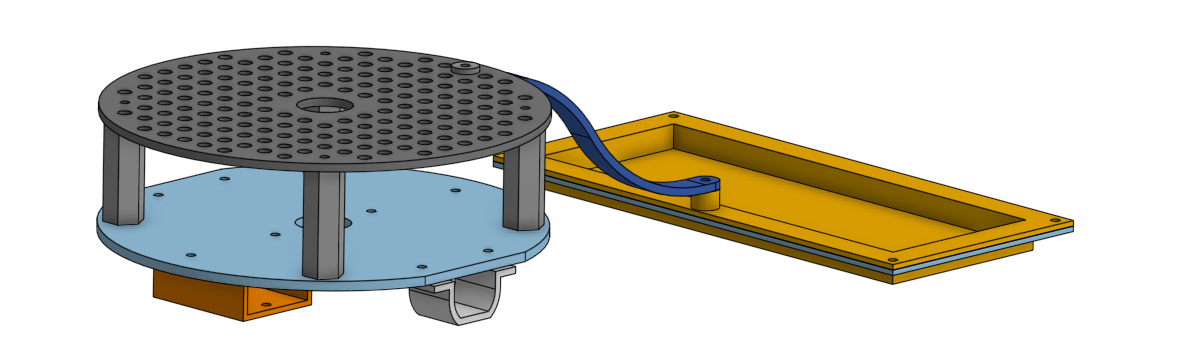
\includegraphics[width=\textwidth, trim={0mm, 8mm, 0mm, 15mm}, clip]{images/my_robot_long.png}}\\
        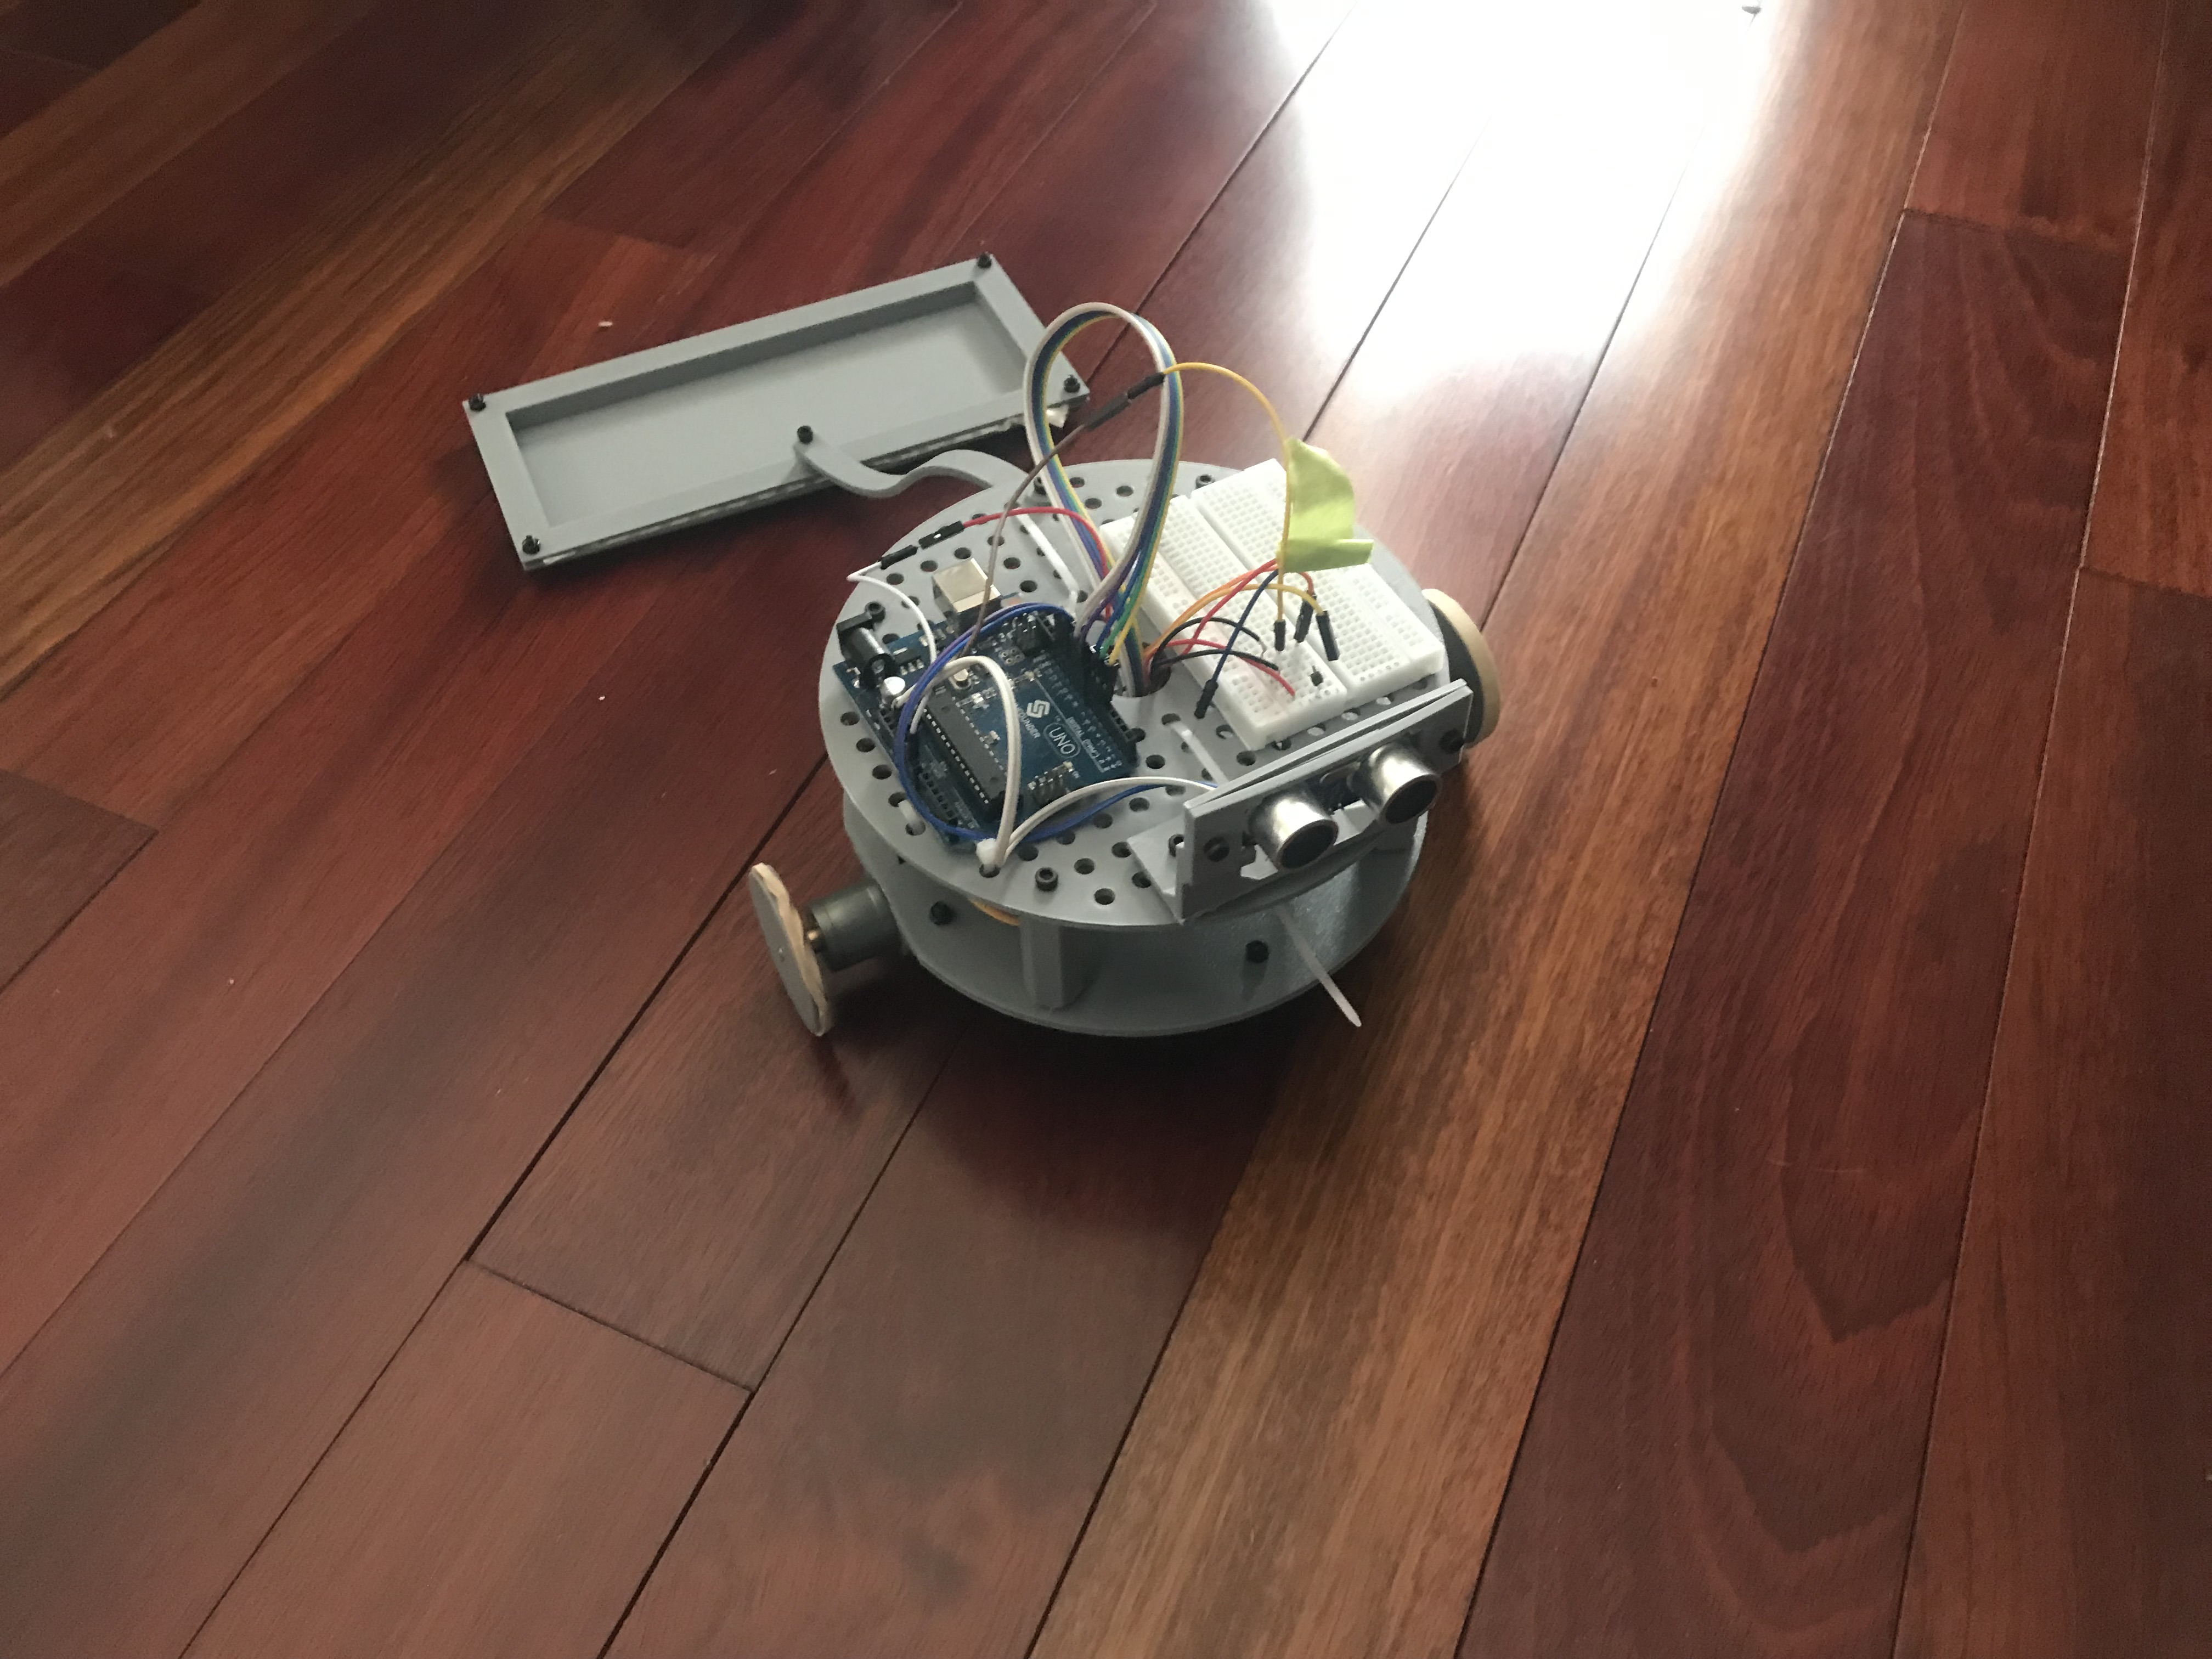
\includegraphics[width=0.43\textwidth, trim={280mm, 340mm, 440mm, 140mm}, clip]{images/mobile_robot.jpg} & 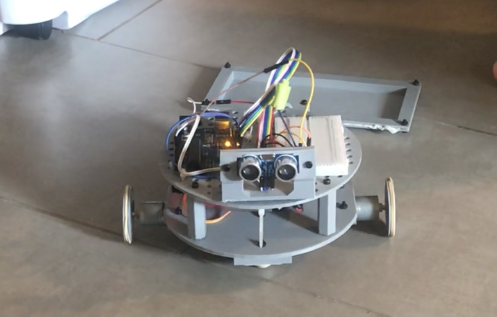
\includegraphics[width=0.57\textwidth, trim={15mm, 8mm, 10mm, 8mm}, clip]{images/my_robot_front.png} \\
    \end{tabular}
\end{center}
\newpage

\section*{Bimanual Force Controlled Robot}
\subsection*{What}
For a research project, I wanted to investigate force control algorithms with the Baxter robot. The Baxter robot is a two-armed robot. Each arm is has $7$ degrees of freedom (DoF). Baxter is different than many other armed robots because its joints are physically elastic for safety, so the arms can be easily over powered. When I started this project, the robot was only able to be controlled through one specific old laptop that came with it. I wanted to get the robot to use its two arms in collaboration to clamp an object with a target force, while moving the object freely throughout space in its workspace.
\subsection*{How}
I started by setting up the robot in a much more convenient way. Forcing users of the robot to develop and run code on a specific computer seemed like a poor situation to me, so I went to reading this robot's documentation. I decided to setup a docker development environment for this system where I installed a $10$ year old version of Linux and the corresponding version of ROS1. In the end, this allowed me to run a single command on an computer I actually wanted to develop on and it was ready. I then implementing a control algorithm by determining where the two arms ends had to be in world space for a given object position in world space. I used the arm separation of the two end effectors to represent the force they were applying, and with a proportional feedback controller I used the system's wrench sensing to make the arms clamp harder when the measured force was less than the target force, and vice versa. Once I knew what end effector positions I wante, I used an inverse kinematics API for the Baxter robot. I tested the code in a Gazebo simulator to safely and quickly test my code before applying it to the physical robot. 
\subsection*{Key Contributions}
\begin{itemize}
    \item \textbf{Docker} was used to make a portable development and deployment environment
    \item \textbf{Gazebo} simulator for ROS was used to safely test and iterate code quickly
    \item A force target was maintained while tracking an arbitrary path within the robots workspace
\end{itemize}
\subsection*{Results}
The main goal of this project was to implement and demonstrate force control for the Baxter robot, and this was acheived as desired. However, making a portable and convenient environment to work with Baxter was also done to make working with this robot much easier. This environment has served as the new way to work with Baxter in the Mechatronics Systems Lab, and is being used by graduate students interested on working with this hardware.

\vspace{0 mm}

\begin{center}
    \begin{tabular}{cc}
        % \multicolumn{2}{c}{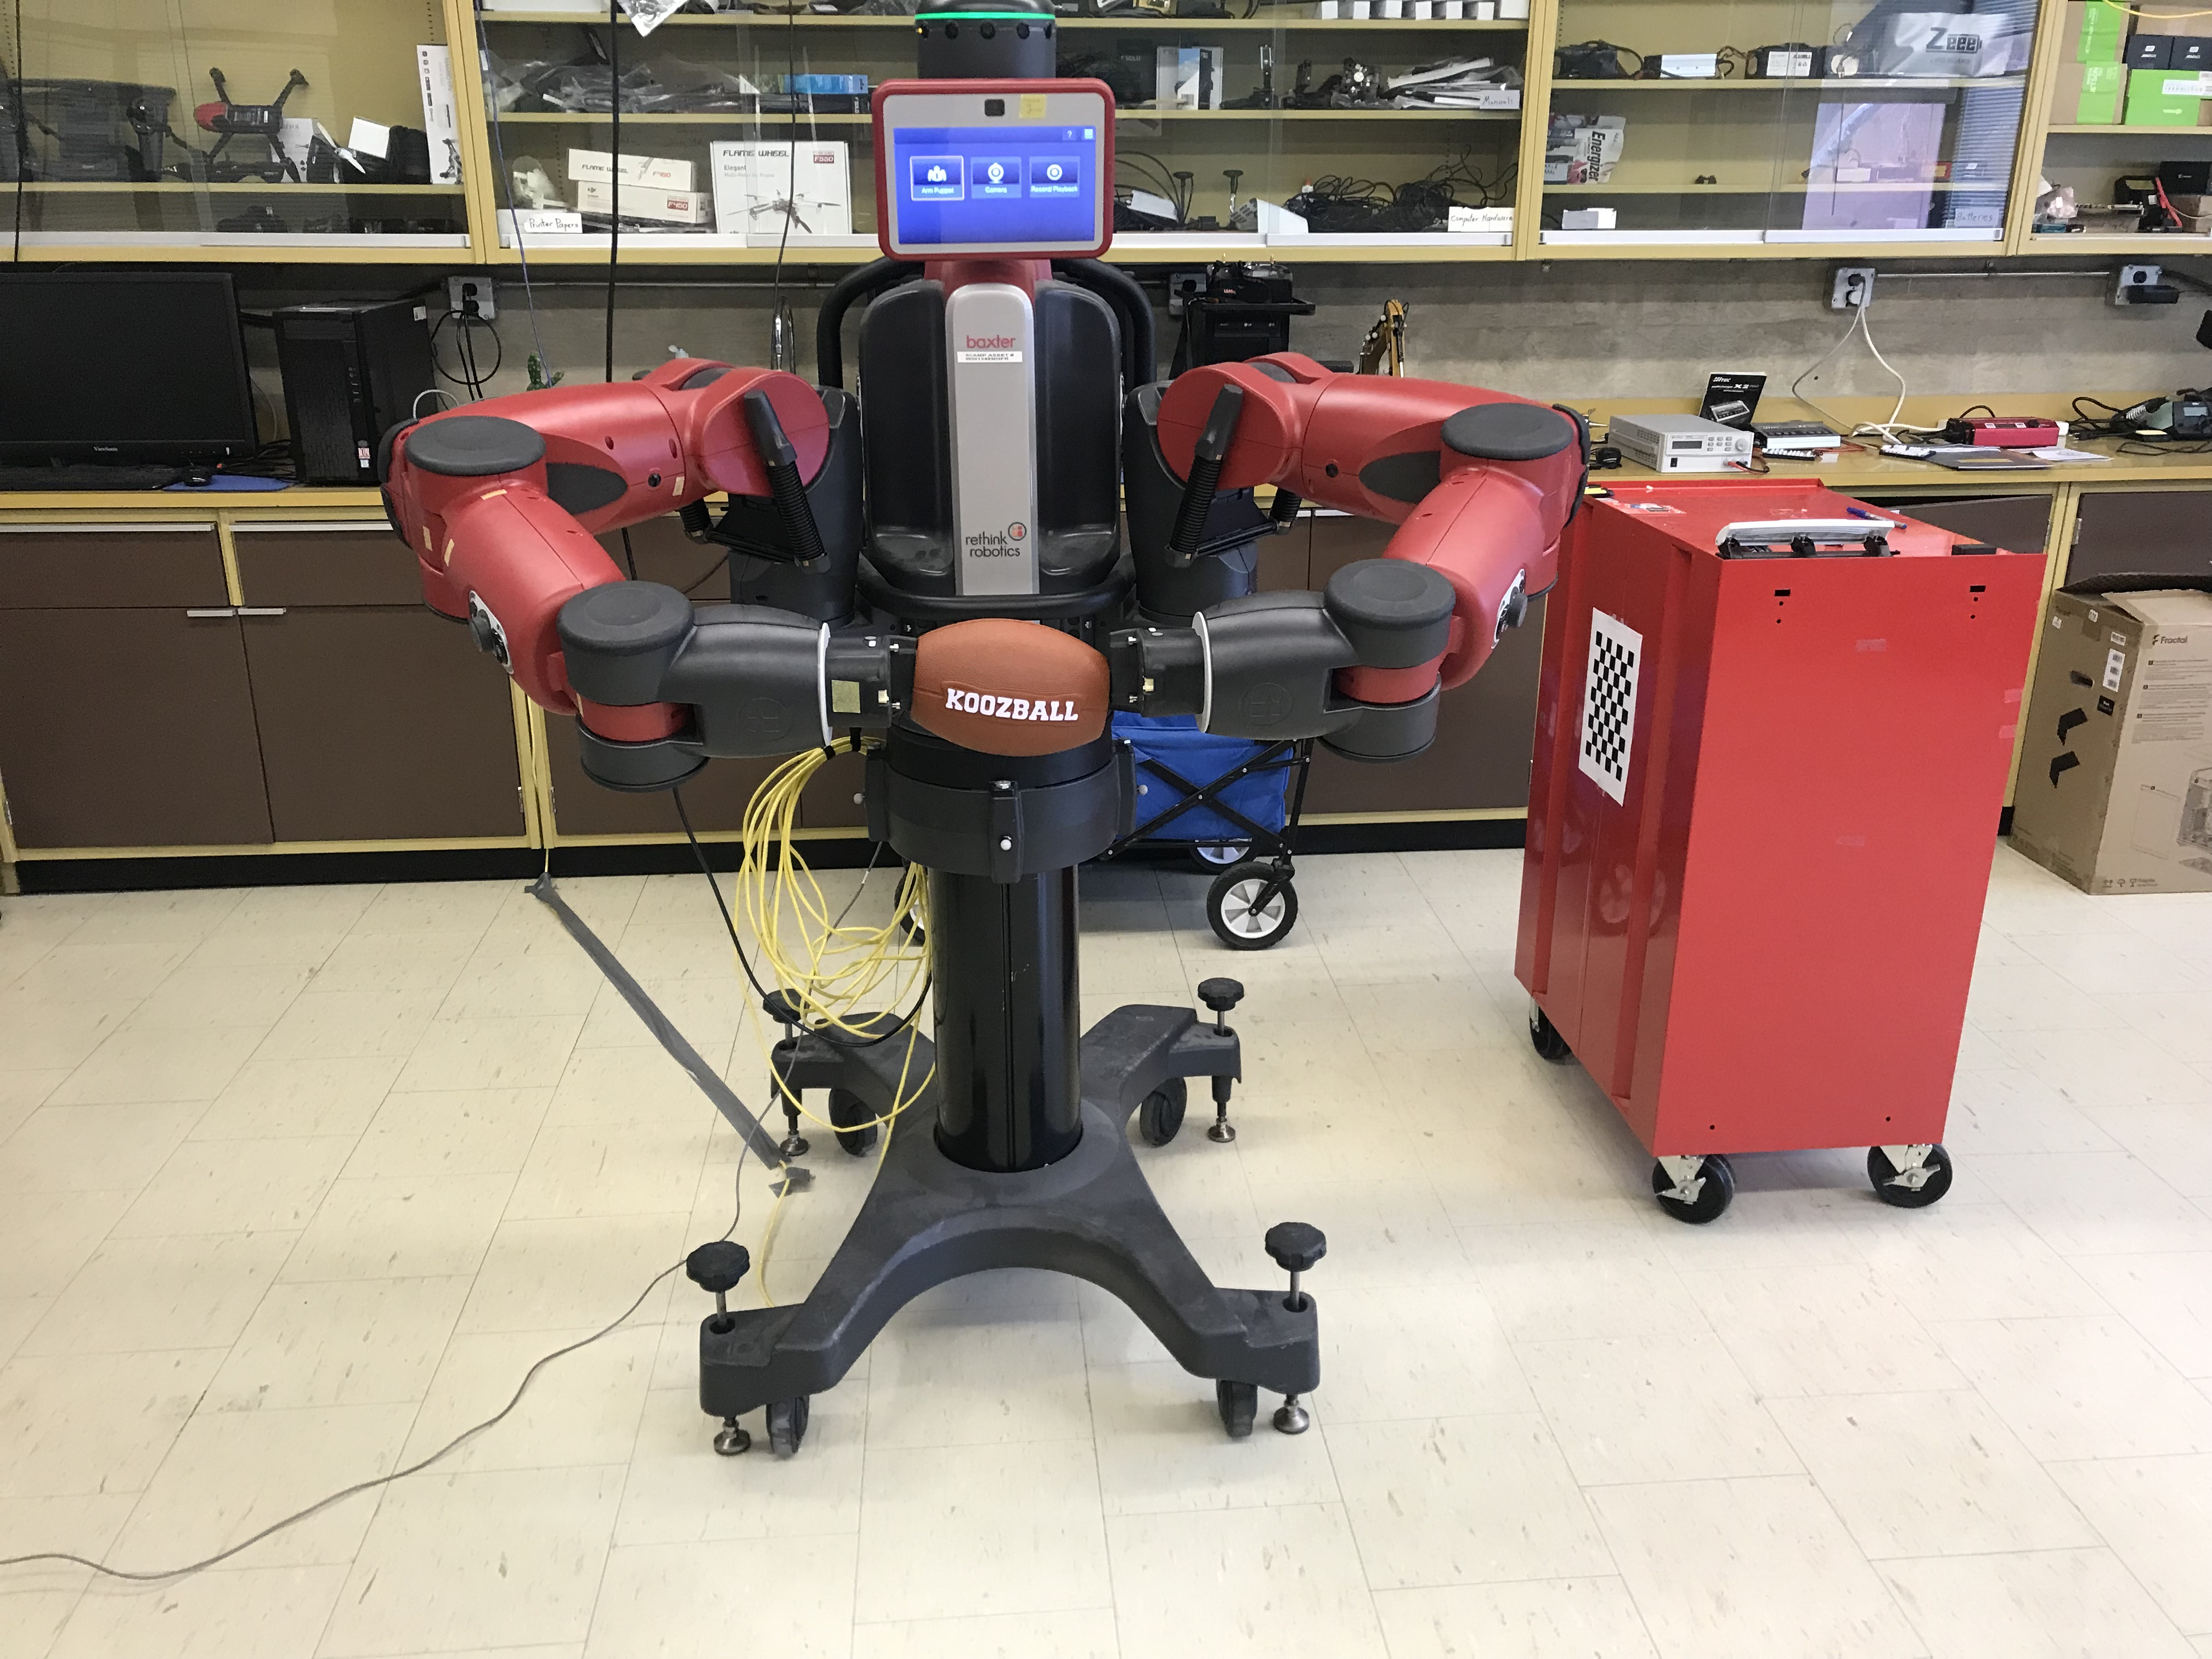
\includegraphics[width=\textwidth, trim={100mm, 480mm, 100mm, 350mm}, clip]{images/baxter_football.jpg}}\\
        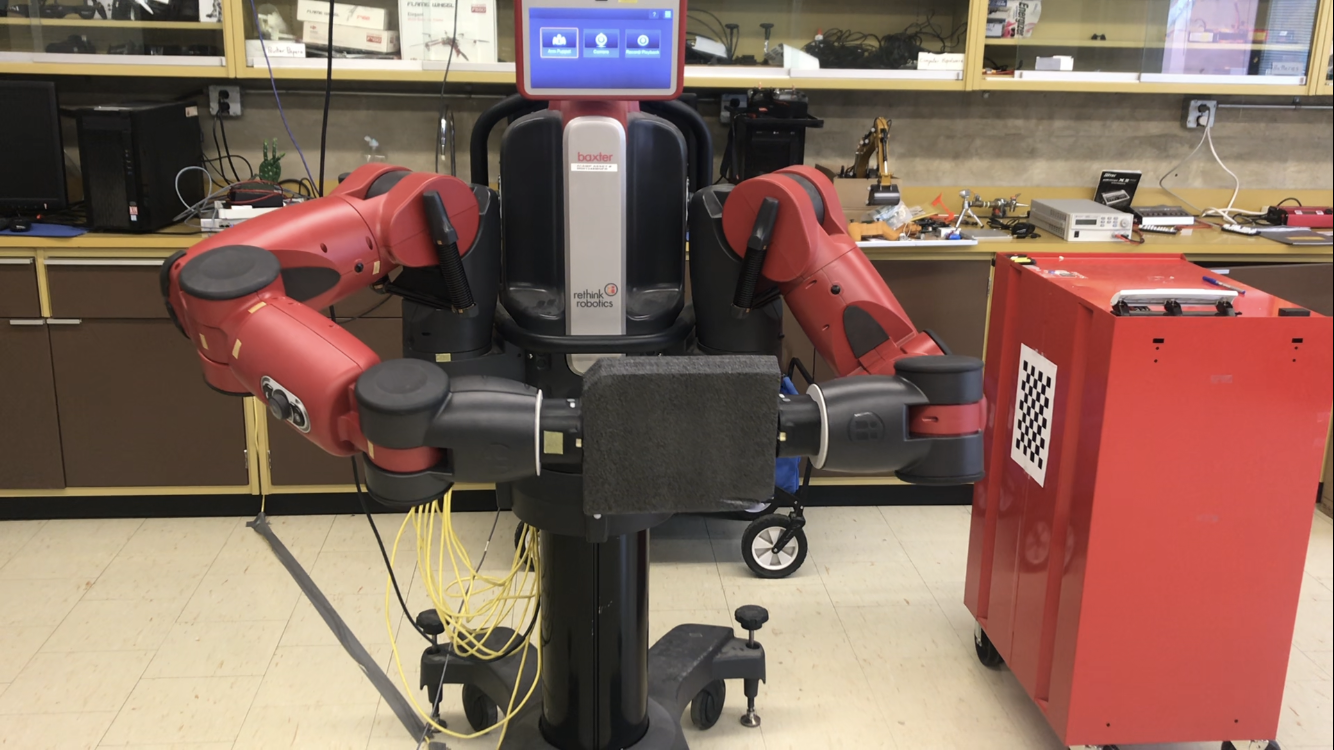
\includegraphics[width=0.6915\textwidth, trim={25mm, 20mm, 60mm, 0mm}, clip]{images/baxter.png} & 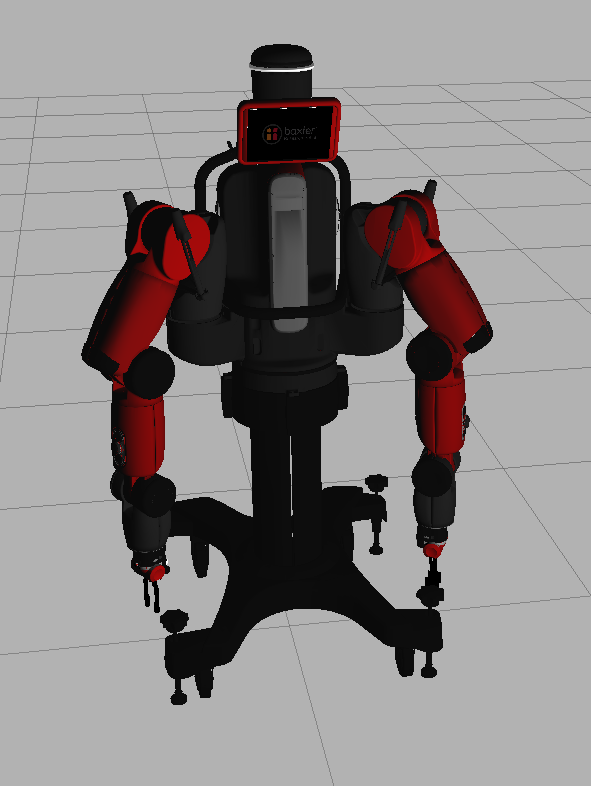
\includegraphics[width=0.3085\textwidth, trim={25mm, 20mm, 30mm, 0mm}, clip]{images/baxter_sim.png} \\
    \end{tabular}
\end{center}
\newpage

\section*{Formula Car Rear Aerodynamic Wing}
\subsection*{What}
The University of Alberta formula SAE team designs and makes a formula style car and races it at an international competition. I lead a mechanical engineering capstone group in the design and manufacturing plan of a full rear aerodynamic wing for their next vehicle. The wing was to use the old iteration as a starting point, and then increase the downforce and lift to drag ratio, and decrease the mass of the device within a given budget. Our team was responsible for designing the profile of the wing to achieve our desired aerodynamic properties as well as the structure and of the wing, and we also decided to implement a drag reduction system (DRS) as well.
\subsection*{How}
In the beginning of this project, I created concepts for our proposed DRS system. I wanted to keep it as simple as possible since the people building the system were going to be undergraduate students. I decided on an externally mounted aluminum linkage system that was powered by a servo hidden inside of the large wing element. The concept was to have the subsystem have two configurations; one where all of the elements were at their optimal angle of attack (AoA), which was based on work from other members, and another where the second and third wing elements were rotated to be facing directly forward. I then modelled all of the hardware (washers, shoulder bolts, bearings, etc.) in SOLIDWORKS parametrically so that the members responsible for the aerodynamics study could easily apply their results to our design. After this I conceptualized, and modelled a rib and spar structure for the main wing element to keep a light weight but rigid structure. All of the structure was verified using Ansys Structural finite element analysis (FEA) software. I also specifically designed for the carbon fiber layup schedule using Ansys Composie PrepPost (ACP) to ensure a suitable but not excessive rigidity and strength.
\subsection*{Key Responsibilities}
\begin{itemize}
    \item \textbf{SOLIDWORKS} was used to parametrically model an entire rear wing, with dynamic configurations following the systems true range of motion
    \item \textbf{Ansys Structural} and \textbf{Ansys Composite PrepPost} were used to verify the strength and rigidity of the system
    \item Lead an engineering team to fully design a rear aerodynamic wing, reallocating man-power and reducing scope as necessary
\end{itemize}
\subsection*{Results}
Compared to the baseline iteration, the rear wing ended up being $21 \%$ lighter when not including the DRS, but even with the new DRS subsystem it was still $14 \%$ lighter. The project used only $77 \%$ of its budget, and was all manufacturing was simple enough to be done by students. The strength of the design was found to have a minimum factor of safety (FoS) of $4$. On top of this, the downforce and lift to drag ratio were also found to have been improved.

\vspace{-6mm}
\begin{center}
    \begin{tabular}{cc}
        \multicolumn{2}{c}{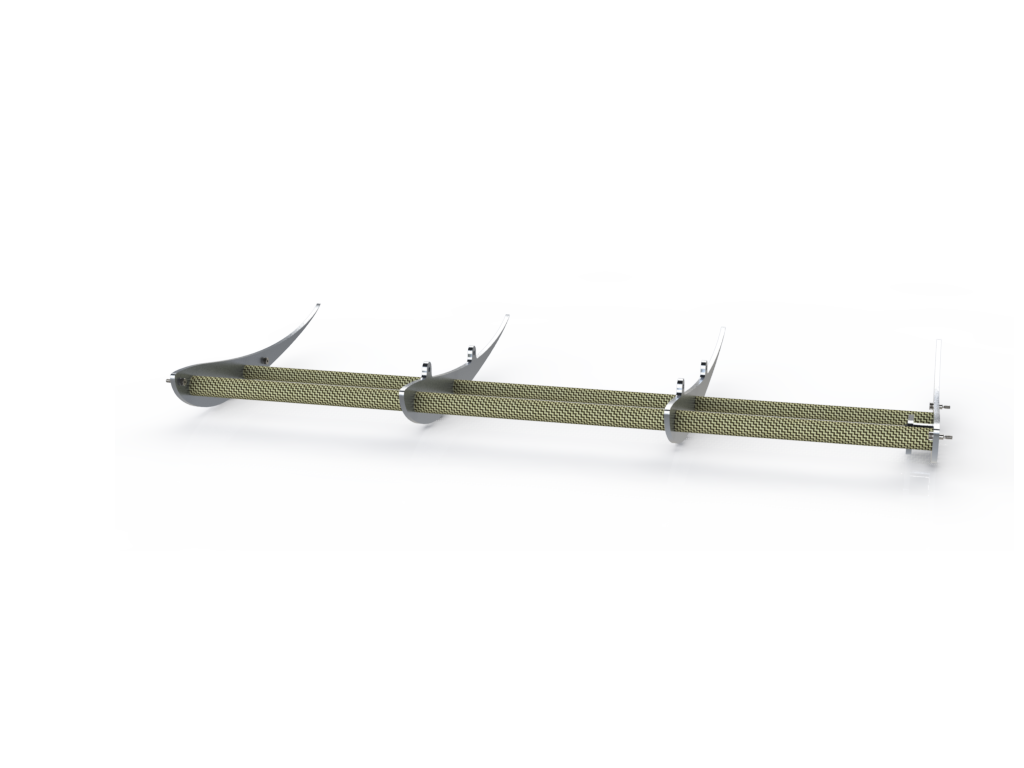
\includegraphics[width=\textwidth, trim={10mm, 25mm, 5mm, 26mm}, clip]{images/rear_wing_skeleton.png}}\\
        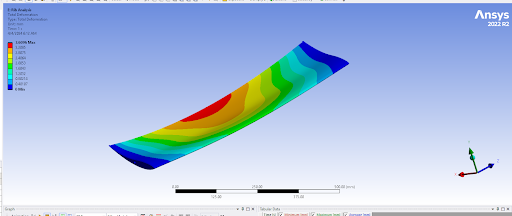
\includegraphics[width=0.51\textwidth, trim={30mm, 5mm, 50mm, 10mm}, clip]{images/rear_wing_fea.png} & 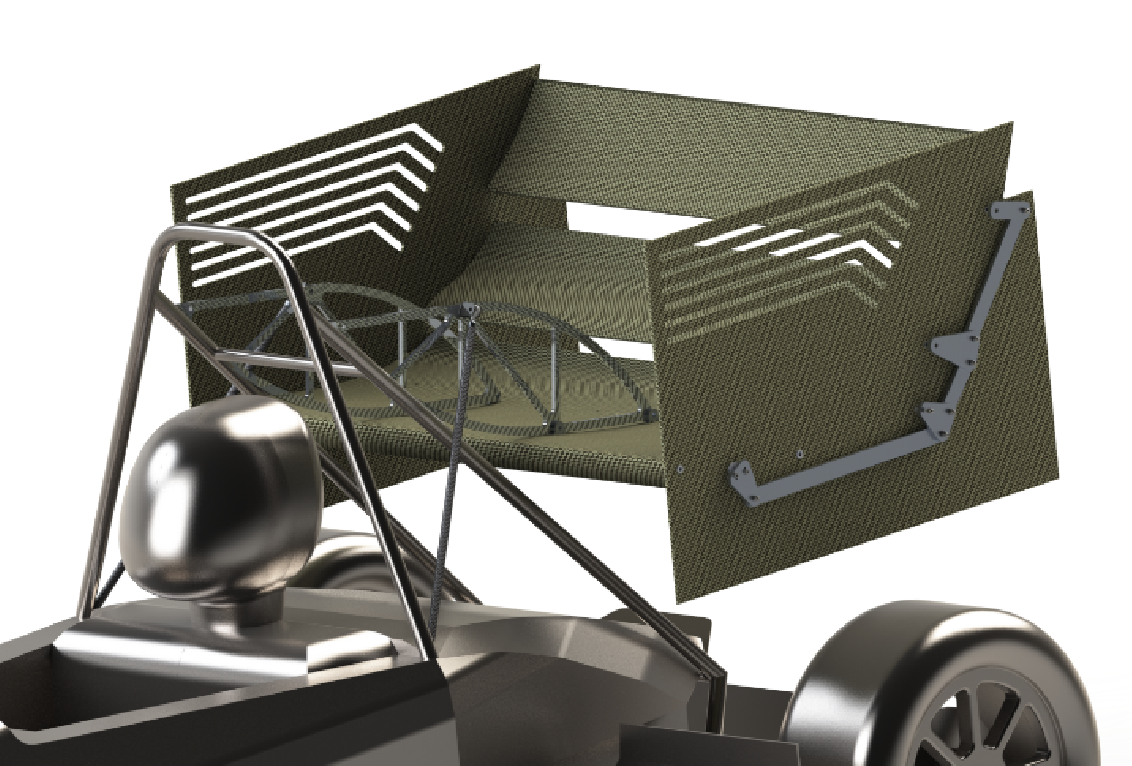
\includegraphics[width=0.49\textwidth, trim={0mm, 0mm, 0mm, 20mm}, clip]{images/integrated_rear_wing.png} \\
    \end{tabular}
\end{center}

\newpage

\end{document}